\documentclass[tikz,border=8pt]{standalone}
% Shared look for every TikZ diagram. Load with \input{../../tools/tikz-style.tex}
\usepackage[T1]{fontenc}
\usepackage{lmodern}
\renewcommand{\sfdefault}{lmr}  % diagrams use the same serif as the text
\usetikzlibrary{arrows.meta, positioning, shapes.geometric, calc, fit, backgrounds}
\definecolor{cblue}{HTML}{4C78A8}
\definecolor{corange}{HTML}{F58518}
\definecolor{cgreen}{HTML}{54A24B}
\definecolor{cred}{HTML}{E45756}
\definecolor{cpurple}{HTML}{B279A2}
\definecolor{cgrey}{HTML}{6B6B6B}
\tikzset{
  every picture/.style={font=\sffamily, line width=1.2pt},
  box/.style={draw=#1, fill=#1!12, rounded corners=4pt, align=center, inner sep=7pt, minimum height=1.1cm},
  box/.default=cgrey,
  arrow/.style={-{Stealth[length=3mm]}, draw=cgrey, line width=1.4pt},
  title/.style={font=\sffamily\bfseries\Large},
  note/.style={font=\sffamily\small, text=cgrey, align=center},
}
\AtBeginDocument{\hyphenpenalty=10000 \exhyphenpenalty=10000}

\begin{document}
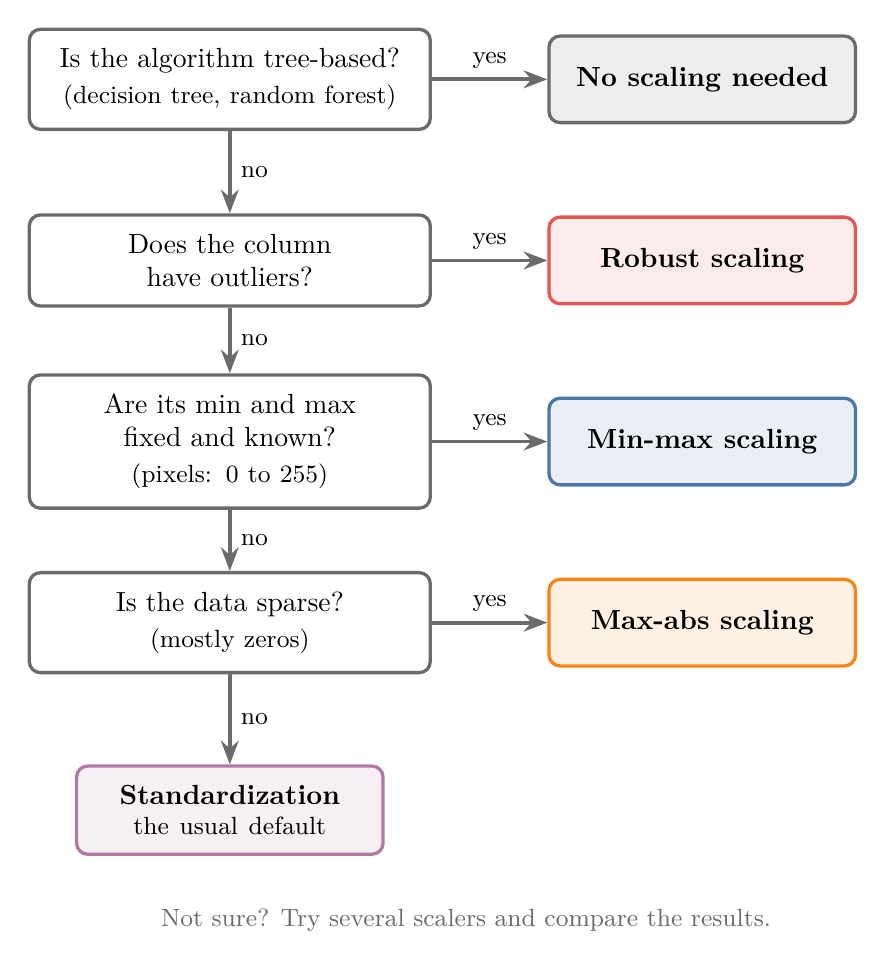
\begin{tikzpicture}[q/.style={box=cgrey, fill=white, text width=4.6cm}, a/.style={box=#1, text width=3.4cm, font=\sffamily\bfseries}]
  \node[q] (q1) at (0,0) {Is the algorithm tree-based?\\[1pt]\small (decision tree, random forest)};
  \node[q] (q2) at (0,-2.3) {Does the column have outliers?};
  \node[q] (q3) at (0,-4.6) {Are its min and max fixed and known?\\[1pt]\small (pixels: 0 to 255)};
  \node[q] (q4) at (0,-6.9) {Is the data sparse?\\[1pt]\small (mostly zeros)};
  \node[a=cpurple, anchor=north] (std) at (0,-8.7) {Standardization\\[-1pt]\normalfont\small the usual default};
  \node[a=cgrey] (no) at (6,0) {No scaling needed};
  \node[a=cred] (rob) at (6,-2.3) {Robust scaling};
  \node[a=cblue] (mm) at (6,-4.6) {Min-max scaling};
  \node[a=corange] (ma) at (6,-6.9) {Max-abs scaling};
  \foreach \f/\t in {q1/no, q2/rob, q3/mm, q4/ma}
    \draw[arrow] (\f.east) -- node[above, font=\sffamily\small] {yes} (\t.west);
  \foreach \f/\t in {q1/q2, q2/q3, q3/q4, q4/std}
    \draw[arrow] (\f.south) -- node[right, font=\sffamily\small] {no} (\t.north);
  \node[note, anchor=north] at (3,-10.4) {Not sure? Try several scalers and compare the results.};
\end{tikzpicture}
\end{document}
